\documentclass[14pt, a4paper]{extarticle}

\usepackage{cmap}
\usepackage{mathtext}
\usepackage[T2A]{fontenc}
\usepackage[utf8]{inputenc}
\usepackage[english, russian]{babel}
\usepackage{indentfirst}
\frenchspacing

\usepackage{amsmath, amssymb, amsfonts, amsthm, mathtools}
\usepackage{icomma}

\usepackage{centernot}
\usepackage{stmaryrd}

\renewcommand{\epsilon}{\ensuremath{\varepsilon}}
\renewcommand{\phi}{\ensuremath{\varphi}}
\renewcommand{\kappa}{\ensuremath{\varkappa}}
\renewcommand{\le}{\ensuremath{\leqslant}}
\renewcommand{\leq}{\ensuremath{\leqslant}}
\renewcommand{\ge}{\ensuremath{\geqslant}}
\renewcommand{\geq}{\ensuremath{\geqslant}}
\renewcommand{\emptyset}{\ensuremath{\varnothing}}

\usepackage{graphicx}
\usepackage{wrapfig}

\usepackage{array, tabularx, tabulary, booktabs}
\usepackage{longtable}
\usepackage{multirow}

\theoremstyle{definition}
\newtheorem{theorem}{Теорема}[section]
\newtheorem{lemma}{Лемма}[section]
\newtheorem{proposition}{Утверждение}[section]
\newtheorem*{exercise}{Упражнение}
\newtheorem{problem}{}

\theoremstyle{definition}
\newtheorem{definition}{Определение}[section]
\newtheorem*{corollary}{Следствие}
\newtheorem*{note}{Замечание}
\newtheorem*{reminder}{Напоминание}
\newtheorem*{example}{Пример}

\theoremstyle{remark}
\newtheorem*{solution}{Решение}

\usepackage{geometry}
\usepackage{setspace}
% \usepackage{enumitem}
\usepackage[inline]{enumitem}
\setlist{leftmargin=25pt}

\geometry{top=20mm}
\geometry{bottom=15mm}
\geometry{left=15mm}
\geometry{right=15mm}

\setlength\parindent{15pt}
\linespread{1.3}

\usepackage{multicol}
\usepackage{soulutf8}

\usepackage{microtype}

\usepackage{tocloft}

\makeatletter
\def\eqref{\@ifstar\@eqref\@@eqref}
\def\@eqref#1{\textup{\tagform@{\ref*{#1}}}}
\def\@@eqref#1{\textup{\tagform@{\ref{#1}}}}
\makeatother
\numberwithin{equation}{section}
\mathtoolsset{showonlyrefs=false}

\usepackage{hyperref}
\usepackage[usenames,dvipsnames,svgnames,table,rgb]{xcolor}
\hypersetup{
    unicode=true,
    colorlinks=true,
    linkcolor=black!15!blue,
    citecolor=green,
    filecolor=magenta,
    urlcolor=NavyBlue,
}

\usepackage{tikz}
\usepackage{tikz-cd}
\usepackage{tkz-euclide}
\usepackage{stackengine}
\usetikzlibrary{angles, babel, quotes}

% \usepackage{paratype}
% \usepackage{euler}

\newcommand{\N}{\ensuremath{\mathbb{N}}}
\newcommand{\Z}{\ensuremath{\mathbb{Z}}}
\newcommand{\Q}{\ensuremath{\mathbb{Q}}}
\newcommand{\R}{\ensuremath{\mathbb{R}}}

\usepackage[normalem]{ulem}
\usepackage{fancyhdr}

\usepackage{graphicx}
\usepackage{wrapfig}
\usepackage{tikz}

\pagestyle{fancy}
\fancyhf{}
\fancyhead[R]{\href{https://vk.com/pr0st0_sasha}{Составитель}}
\chead{\textbf{Приемка ФПМИ 2023}}

% ---------

\begin{document}

\subsection*{Задачи по информатике}

\begin{problem}
    Дан отсортированный массив целых чисел, вывести 
    отсортированный массив их квадратов.
\end{problem}

\begin{problem}
    Построй очередь на двух стеках.
\end{problem}

\begin{problem}
    Двое играют в игру: нужно по очереди класть на прямоугольный
    стол пятирублевые моненты. Если один не может положить 
    монету, то победа засчитывается второму.

    Может ли какой-то из игроков гарантированно победить? Если может,
    то предложи стратегию.
\end{problem}

\begin{problem}
    Биба и Боба прогневали короля. Им грозит смертная казнь.
    Однако правитель в этой стране милосердный. Он предложил
    им следующее: их ведут в темницу и разводят по одиночным камерам,
    там они бросают монетку, а далее каждый должен сказать,
    что выпало у товарища. Если хотя бы один угадывает, их отпускают, 
    иначе ...

    У товарищей есть пару минут, пока их ведут в камеры, чтобы 
    обсудить стратегию. Итак вопрос: смогут ли они гарантированно выйти
    живыми и невредимыми?
\end{problem}

\begin{problem}
    Имеется бинарное дерево, состоящее из целых чисел.
    Требуется найти в нем путь (может начинаться и 
    заканчиваться в любой ноде) с максимальной суммой.

    \textit{Предложить решение за линию.}

    // Вставить картику с деревом
\end{problem}

\begin{problem}
    Принц-Полукровка оставил в своем учебнике по зельеварению 
    огромное число подсказок и заметок. Одна из заметок содержала 
    "Закон несохранения массы". Далее идет ее текст.

    \textit{Посмотрим на веса каждого из ингредиентов в рецепте и 
    каждому из них сопоставим столбик единичной ширины и высоты, 
    равной числу граммов соответствующего ингредиента. 
    Выровняем их снизу по одной линии и получим "гистограмму 
    ингредиентов". Тогда масса полученного зелья будет равняться 
    площади самого большого прямоугольника в гистограмме, одна 
    из сторон которого лежит на общей нижней линии.}
\end{problem}

\begin{problem}
    Есть односвязный список, состоящий из различных значений. 
    Возможно в нем есть цикл. Опиши алгоритм, который находит
    начало этого цикла, а если цикла нет --- выводит \textit{-1}.

    \begin{tikzpicture}[->,>=stealth,shorten >=1pt,auto,
        node distance=2.5cm, thick,
        main node/.style={circle,draw,font=\sffamily\Large\bfseries}]

    % Nodes
    \node[main node] (1) {1};
    \node[main node] (2) [right of=1] {4};
    \node[main node] (3) [right of=2] {2};
    \node[main node] (4) [right of=0.5cm of 3, above of=3] {3};
    \node[main node] (5) [right of=4, below of=4] {5};
    \node[main node] (6) [below of=4, below of=4] {6};

    % Edges
    \path[every node/.style={font=\sffamily\small}]
    (1) edge (2)
    (2) edge (3)
    (3) edge (4)
    (4) edge (5)
    (5) edge (6)
    (6) edge (3);

    \end{tikzpicture}
\end{problem}

\begin{problem}
    Вагоны новой кольцевой железной дороги было предложено расписать 
    $N$ дизайнерам. Каждый дизайнер выбирал для своей раскраски полосу 
    длиной $L_i$, начинающуюся от начала вагона и гарантированно 
    помещающуюся на вагоне. Тем самым какие-то работы были полностью 
    закрашены, а какие-то всё же были видны хотя бы частично.

    Тебе дана последовательность перекраски. После завершения работы 
    каждого дизайнера выведите одно число — количество различных работ, 
    элементы которых видны на момент завершения.

    \textit{Предложить решение за линию.}
\end{problem}

\begin{problem}
    \textbf{Король и вино.}

    Представь, ты --- король, и у тебя завтра день рождения. По такому случаю ты устраиваешь
    вечеринку! Но какая же вечеринка может обойтись без открытия винного погреба?)
    И вот ты спускаешься в свой погреб и обнаруживаешь в нем ... записку, в которой говорится,
    что одна из 1000 бутылок вина отравлена. Яд этот очень опасный и всего одна его капля
    способна убить человека всего за 15-20 часов. И всё бы было не так плохо, да вот до праздника
    остается всего один день! 
    
    Подвергать риску себя и своих гостей ты не можешь, зато у тебя 
    в темнице множество узников, которые ждут своей казни. И ты решаешь дать им вина,
    чтобы вычислить отравленную бутылку. Человек ты сердобольный, поэтому тебе хочется подвергнуть
    риску как можно меньшее количество заключённых. Вопрос: какое минимальное количество 
    заключённых должно попробовать вино из бутылок, чтобы точно найти отравленную в течение 24 часов?
\end{problem}

\begin{problem}
    \textbf{Infinity Train}

    Представь замкнутую по окружности железную дорогу. 
    По ней едет поезд, последний вагон которого скреплён с первым так, 
    что внутри можно свободно перемещаться между вагонами. 
    Ты оказался в каком-то случайном вагоне и твоя задача — \textit{посчитать 
    их общее количество}. В каждом вагоне можно включать или выключать 
    свет, но начальное положение переключателей случайное и заранее неизвестно.

    Все вагоны внутри выглядят одинаково, окна закрыты так, что невозможно 
    посмотреть наружу, движение поезда равномерное. Помечать вагоны как-либо, 
    кроме включения или выключения света, нельзя. 
    Количество вагонов конечно (не верьте заголовку).

    \textit{Придумать решение за логарифм.}
\end{problem}

% -------
\subsection*{Задачи по математике}
\setcounter{problem}{0}

\begin{problem}
    Можно ли торт 3 разрезами поделить на 8 частей.
\end{problem}

\begin{problem}
    В кубической комнате со стороной 2 летают 9 мух. 
    Докажи, что найдется хотя бы одна пара мух, 
    находящихся на расстоянии не большем $\sqrt{3}$.
\end{problem}

\begin{problem}
    У шахматной доски отрезали два противолежащих уголка.
    Можно ли теперь покрыть ее доминошками (по структуре они
    наполовину черные, наполовину белые)?
\end{problem}

\begin{problem}
    Решить $3\sqrt{4x - 5y + 7} +
    5|3x - 4y + 6| \leqslant 4$, где $x, y \in \Z$.
    В ответе указать $max(x+y)$.
\end{problem}

\begin{problem}
    \textbf{Читать голосом Александра Пушного.}

    В эфире самая смешивательная среди взбалтывательных и самая
    взбалтывательная среди смешивательных рубрик программы <<Галилео>>, 
    которая называется ЭЭЭЭЭЭКСПЕРИМЕНТЫ.
    
    Друзья, смотрите, мы берем две совершенно одинаковые кружки.
    В одной из них молоко, в другой --- кофе (в одинаковых количествах). 
    Переливаем ложку молока в кофе, перемешаем, 
    а затем обратно переливаем ложку получившейся смеси в стакан с молоком. 
    Итак, наши внимательные зрители, чего же у нас оказалось больше:
    молока в кофе или кофе в молоке?

    \textit{Подсказка}. Можешь для начала решить следующую задачу:

    На главную туристическую площадь приехали два туристических 
    автобуса. Все места в каждом из автобусов были заняты. 
    В первом автобусе находилось 20 польских 
    туристов, во втором --- 20 чешских. Во время экскурсии 
    начался ливень, и туристы бросились в автобусы, не разбирая, где чей. 
    Кого больше: чешских туристов в польском автобусе или польских 
    туристов в чешском?
\end{problem}

\begin{problem}
    Существует ли такой $x$, что $tg(x) + \sqrt{3}$ и 
    $ctg(x) + \sqrt{3}$ целые числа?
\end{problem}

\begin{problem}
    //Жду Федю с картинкой про геому 7 класс
\end{problem}

\begin{problem}
    Решить $2x \cdot 2^x + 3x \cdot 3^x + 1 \geqslant 
    \sqrt{4^x + 9^x +1} \cdot \sqrt{13x^2 + 1}.$
\end{problem}

\begin{problem}
    //Жду Федю с картинкой про геому 4 решения
\end{problem}

\begin{problem}
    Доказать иррациональность $\sqrt{2}$ (\textit{несколькими способами}).
\end{problem}

\begin{problem}
    \begin{multicols}{2}
        Из 9 аксиом поля действительных чисел вывести следующее:
        \renewcommand{\labelenumi}{\alph{enumi})}
        \begin{enumerate}
        \item $\forall a \in \R \ \exists ! \; (-a)\in \R : a + (-a) = 0;$
        
        \item $\forall a \in \R : \ a \cdot 0 = 0;$
        
        \item $\forall a \in \R : \ (-1) \cdot a = -a.$
        \end{enumerate}

        \columnbreak

        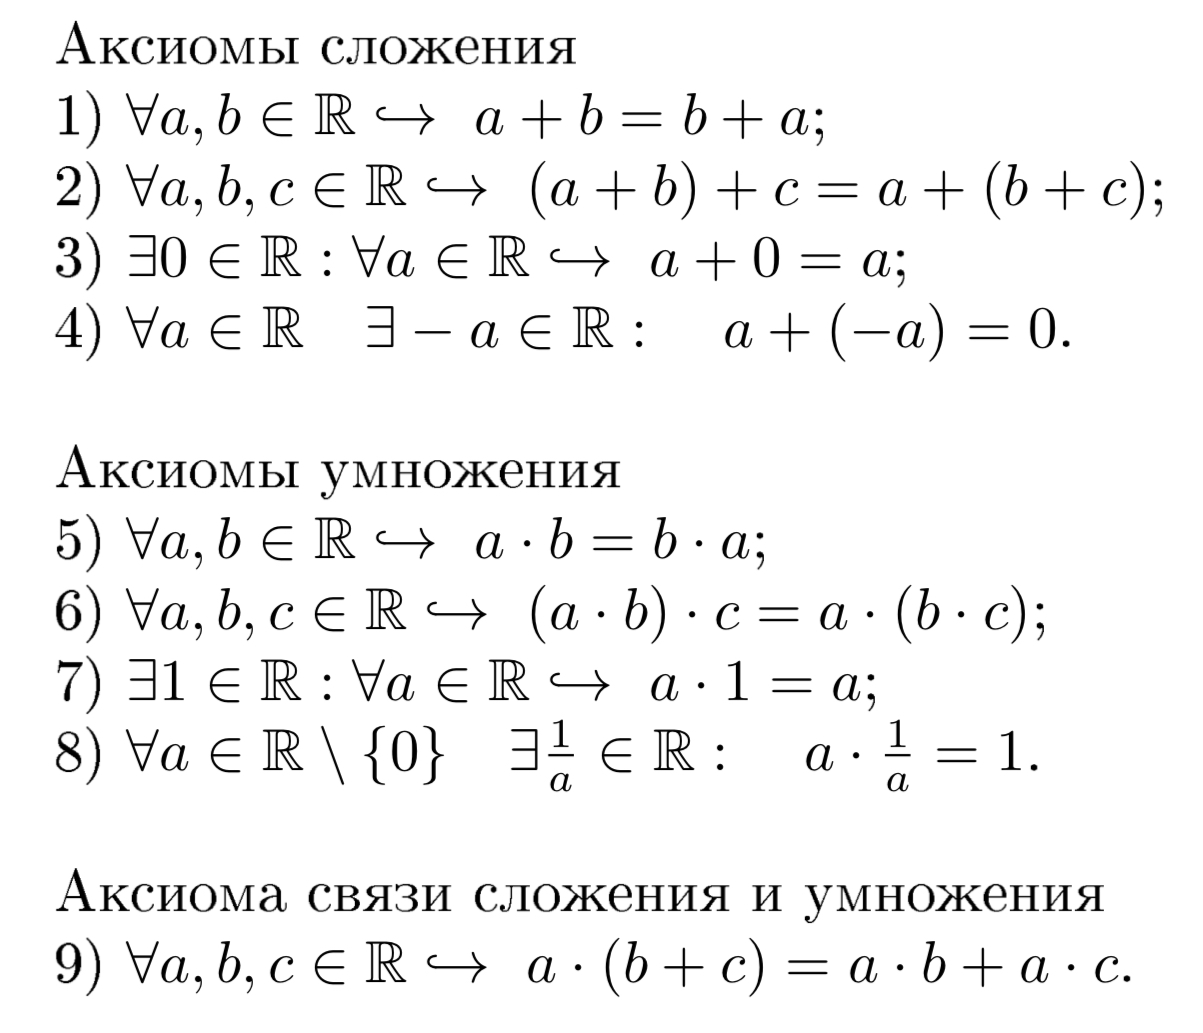
\includegraphics[width=0.46\textwidth]{ax.jpeg}
      \end{multicols}
\end{problem}

\begin{problem}
    Доказать счетность/несчетность следующих множеств:
    \renewcommand{\labelenumi}{\alph{enumi})}
    \begin{enumerate*}[before=\hspace{1ex}, itemjoin=;\hspace*{3ex}]
        \item \Z
        \item \Q
        \item \R
    \end{enumerate*}
\end{problem}

\begin{problem}
    Доказать, что $\displaystyle\lim_{n\to\infty}{\sqrt[n]{n}} = 1.$
\end{problem}

\begin{problem}
    Доказать, что $D(x) = \displaystyle\lim_{m\to\infty}{\lim_{n\to\infty}
    {\cos^{2n}(\pi \cdot m! \cdot x)}}$, где $D(x)$ - функция Дирихле.
\end{problem}

\begin{problem}
    \textbf{Бонус к первой задаче.}

    Докажите, что в $\R^2$ это невозможно.

    Здесь торт --- связное выпуклое множество в $\R^2$ 
    с топологией, порождённой евклидовой метрикой.
\end{problem}

\newpage
\section*{Решения}
\subsection*{Информатика}
\setcounter{problem}{0}

\begin{problem}
    Идейно: самые большие по модулю числа на концах.

    \textit{leftIndex = 0, rightIndex = n - 1;}

    Дальше сравниваем элементы и записываем в новый массив с конца.
\end{problem}

\begin{problem}
    stackIn, stackOut.
\end{problem}

\begin{problem}
    Идея симметрии. Первый кладет монету на центр стола, второй кладет
    куда-то, а задача первого --- симметрично отражать ходы соперника.
\end{problem}

\begin{problem}
    \textit{Подсказка.} От чего можно отталкиваться, если не знаешь, 
    что выпало у соседа?

    Один говорит, что выпало у него, второй --- отрицание своего результата.
\end{problem}

\begin{problem}
    Через DFS посчитать максимальные пути 
\end{problem}

\begin{problem}
    затехать
\end{problem}

\end{document}